%main for analyse

\part{System Analysis}
\label{system_analysis}

\chapter{Description of Water Supply Systems}
\label{description_of_water_supply_systems}

 \emph{This chapter gives a general overview of hydraulic systems and an introduction to the WSS in Randers. The basic topology and structures of water supply networks are explained. }

\section{Hydraulic system overview}
\label{hydraulic_system_overview}

WSSs are designed to deliver water to consumers in terms of sufficient pressure and appropriate chemical composition. Distribution systems as such are typically transport water from one geographical place to another. In practice, there are different methods existing to achieve this water transport. One example is to make use of natural advantages such as the water stored in mountains, and therefore use the potential energy to provide pressure in the network. Good examples are countries like Norway and Sweden where the advantages of the landscape can be exploited. However, in this project the origin of the water is considered as groundwater, considering that in Denmark all reservoirs in the network are tapping water from the ground. After tapping the water, it goes through a cleaning process at the waterwork and afterwards the pure water is pumped into the network \cite{prahata}. In WSSs, pumps and valves are the elements that enable the delivery of water to the consumers or to elevated reservoirs, storing water for later use. Such a network is illustrated in the figure below: 

%illustration of WSS
\begin{figure}[H]
\centering
\includegraphics[width=0.35\textwidth]{report/pictures/missingfigure}
\caption{Illustration of a WSS.}
\label{fig:WSS_example}
\end{figure}

The delivered water needs to fulfil a certain pressure criteria in order to reach consumers at higher levels. For example, in some cases the pressure has to be high enough to make it to the fourth floor of a building and still provide appropriate pressure in the water taps. In such cases, generally booster pumps are placed in the area, helping to supply pressure. Too large pressure values however  increase water losses due to pipe waste \cite{walski2003advanced}.

Another criteria is that the flows through particular pipes need to stay within acceptable limits. A low flow rate can lead to water quality problems due to the undesirable microorganisms in the water and due to the metal and salt accumulation on the wall of the pipes \cite{walski2003advanced}. 

As can be seen in \figref{fig:WSS_example}, typically WSSs consist of pipe, valve, reservoir, elevated reservoir(tank) and pump components. The common property of these components is that they are all two-terminal components, therefore they can be characterized by the dynamic relationship between the pressure drop across the two endpoints and the flow through the elements \cite{master_aau}. 

\subsection{Pipe system}
\label{pipe_system}

Pipes are the most common components of WSSs since they are used for carrying pressurized water. They serve as a connection between components. The network can be separated into different subsections, concerning the physical size and purpose of the pipes. Water supply networks consist of transmission mains, arterial mains, distribution mains and service lines as shown in the example below: 

%illustration of pipe topology / loop configuration
\begin{figure}[H]
\centering
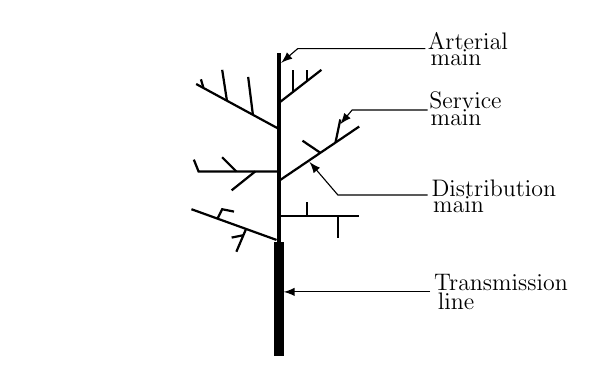
\begin{tikzpicture}[scale=0.6,transform shape]

\fill [black] (0.1,0.1) rectangle (0.3,2.5);
\fill [black] (0.15,6.5) rectangle (0.25,2.5);

\draw [thick](0.15,2.55) -- (-1.65,3.2);
\draw [thick](-0.5,2.77) -- (-0.7,2.3);
\draw [thick](-0.55,2.65) -- (-0.8,2.6);
\draw [thick](-1.1,3) -- (-1,3.2) -- (-0.75,3.15);
\draw [thick](0.2,3.05) -- (1.9,3.05);
\draw [thick](0.8,3.05) -- (0.8,3.35);
\draw [thick](1.45,3.05) -- (1.45,2.6);
\draw [thick](0.2,4) -- (-1.5,4) -- (-1.6,4.25);
\draw [thick](-0.3,4) node (v1) {} -- (-0.8,3.6);
\draw [thick](v1);
\draw [thick](-0.7,4) -- (-1,4.3);
\draw [thick](0.2,3.8) -- (1.9,4.95);
\draw [thick](1.4,4.62) -- (1.5,5.1);
\draw [thick](1.07,4.4) -- (0.7,4.65);
\draw [thick](0.2,4.9) -- (-1.55,5.85);
\draw [thick](-0.35,5.2) -- (-0.45,6);
\draw [thick](-0.9,5.5) -- (-1,6.15);
\draw [thick](-1.4,5.78) -- (-1.45,5.95);
\draw [thick](0.2,5.45) -- (1.1,6.15);
\draw [thick](0.8,5.92) -- (0.8,6.15);
\draw [thick](0.5,5.69) -- (0.5,6.15);
%\draw [-latex](3.4,1.45) -- (0.3,1.85);
\node at (4.9,1.65) {\Large Transmission};
\node at (3.95,1.25) {\Large line};
%\draw [-latex](3.35,3.4) -- (0.6,4.05);
\node at (4.75,3.65) {\Large Distribution};
\node at (4,3.3) {\Large main};
\node at (4.15,5.5) {\Large Service};
\node at (3.95,5.15) {\Large main};
\node at (4.2,6.75) {\Large Arterial};
\node at (3.95,6.4) {\Large main};
%\draw [-latex](3.25,5.25) -- (1.5,5);
%\draw [-latex](3.2,6.55) -- (0.25,6.4);
\node at (-5,3.6) {         };
\draw [-latex](3.3,6.6) -- (0.6,6.6) -- (0.25,6.3);
\draw [-latex](3.35,5.3) -- (1.75,5.3) -- (1.5,5);
\draw [-latex](3.35,3.5) -- (1.45,3.5) -- (0.85,4.2);
\draw [-latex](3.4,1.45) -- (0.3,1.45);
\end{tikzpicture} 
\caption{Illustration of pipe mains. Tree configuration.}
\label{fig:pipemain_example}
\end{figure}

Transmission mains deliver large amounts of water over long distances. Arterial and distribution mains provide intermediate steps towards delivering water to the end-users. Service lines transmit the water from the distribution mains straight to the end-users \cite{grigg2012water}.

The transmission and distribution network can have a topology that is called a loop or a tree structure. \figref{fig:pipemain_example} shows an example for a tree configuration. This type of configuration is most frequently found in rural areas \cite{mays}. Typically the network has only one path for water to reach the end-users. Common problems with this configuration is that on the outer parts of the system lower pressures can be experienced due to the pressure losses from long flow paths. The flow dynamics within this kind of systems therefore consist of large flows closer to the source that turns into smaller flows on the outer parts of the system. Main disadvantage of a purely tree structure system is that due to maintenance or momentary breakdowns, the system suffers disruption of service \cite{mays}. 

Loop networks have a configuration as shown in \figref{fig:loop_configuration}. 

%illustration of loop configuration
\begin{figure}[H]
\centering
\includegraphics[width=0.35\textwidth]{report/pictures/missingfigure}
\caption{Loop configuration.}
\label{fig:loop_configuration}
\end{figure}

Loop networks are usually composed of smaller loops which made up of smaller distribution mains, and larger loops that are connected to arterial or transmission mains. Elevated reservoirs are typically placed in the centre of the system due to pressure losses resulting from flows through the loop network \cite{council2007drinking}. In the presence of the larger loops, they may be used to feed an internal distribution grid or a distribution grid attached to the outer part of the loop. Loop configurations are generally associated with larger suburban and city distribution systems such as the WSS in Randers\cite{council2007drinking}. 

\subsection{Elevated reservoirs}
\label{elevated_reservoirs}

Elevated reservoirs are typically placed in the system to use them as buffers and level out the pressure and flow demand differences. When the demand is high, the waterworks might not be able to provide the sufficient amount of water in the network. In these cases, the elevated reservoir supplies the remaining demand to the network. When the user consumption decreases, the system can be controlled such that the tank is being refilled to provide the required demand for the next peak. Having such an elevated reservoir in the network, the system becomes more independent of the pump stations, as the refilled tank can itself maintain the desired pressure and flow for a limited time. 

Due to the elevation of the tank, when it is filled up, the pumping stations need to provide a pressure higher than the pressure in the water tank. Therefore when the tank is being emptied, the pumping stations can reduce the amount of pressure they provide to the system, since the pressure from the elevated reservoir becomes dominant. This is due to that the dynamics of systems with large storages come primarily from the pressure of the tank(cite). This is due to the height change of the tank being very slow because of the large diameter of the tank. For these considerations, the effect of these elevated reservoirs has to be taken into account while modelling the system. 

\subsection{Pumps}
\label{pumps}



\subsection{Valves}
\label{valves}

\section{The Randers water supply network}
\label{the_randers_water_supply_network}



%\section{Setup Considerations}

% This section should contain to things. 

% 1: Req. for water pressure 
% 2: Constrain about water quality 








 
 

\chapter{Requirements and Constraints}
\label{Requirements_and_constraints}

This section is not defined yet. 

\chapter{Network simplification}
\label{network_simplification}

\emph{This chapter gives a general introduction about the need for model simplification in WSSs. Different approaches and methods are discussed in a state of art manner, including the development and methodologies employed in this field. Lastly, an attempt is made to simplify the Randers WSS, using one of the techniques which are being introduced in this chapter. }

\section{Purpose of the model reduction}
\label{purpose_of_the_model_reduction}

As it was explained in \chapref{description_of_water_supply_systems}, the typical components of WSSs are reservoirs, pipes, pumps and valves. Each of these interconnected elements are dependant on their neighbours, thus the behaviour of the entire WSS depends on each of its elements. For simulation purposes, it is required that the model of the real-life network consists of thousands of elements in order to accurately replicate hydraulic behaviour and the topographical layout of the system. Such models are appropriate for simulation purposes, however, online optimisation tasks are much more computationally demanding, therefore simplified models are required. There are different approaches for model reduction, however the outcome of most of these methods is a hydraulic model with a smaller number of components than the original one. 

The use of Geographic Information Systems(GIS) in the water industry resulted in an increasing amount of information about actual network topology and service that can be utilized in a model \cite{johnson2016geographic}. As a consequence this, normally the simulation model of the WSSs include exactly the same amount of components as in real-life, and therefore a large-scale system is defined. 

The efficiency and accuracy of large-scale system reduction highly depend on the model complexity and the selected method. Several research in this field has been focusing the verification of the different methods and therefore provided case studies for the different approaches. 

\section{State of the art model reduction analysis}
\label{state_of_the_art_model_reduction_analysis}

In the frame of this project, the WSS in Randers is considered as a large-scale system and attempted to be reduced. However, before discussing the reduction on the actual model network, first the different methods for model reduction are introduced in a state of the art manner. It is worth noting that throughout the report, the terms reduction and simplification are used alternately to describe of process of achieving a hydraulic model with a smaller number of components than the original. The different reduction approaches, discussed in this report are: 

\begin{itemize}
\item Skeletonization, which were researched in \cite{walski2003advanced} and \cite{battlepaper}.
\item Parameter fitting (cite)
\item Graph decomposition (cite)
\item Variable elimination (cite)
\end{itemize}

\subsection{Skeletonization}
\label{skeletonization}

Skeletonization can be considered as a reduction of data needed to represent the operation of the hydraulic system without significant loss of information \cite{reduction_PHD}. The basic types of network components are maintained but the individual network components are combined and replaced. Skeletonization is not a single process but several different low-level element removal processes that must be applied in series in order to ensure that the demands in the network are logically reduced back to their source of supply. 

\subsection{Parameter fitting}
\label{parameter_fitting}

(in progress)

\subsection{Graph decomposition}
\label{graph_decomposition}

(in progress)

\subsection{Variable elimination}
\label{variable_elimination}

(in progress)





















